\chapter{Отримання різноманітних картин на екрані осцилографа} 
\label{chapter:first}

\section{Одноканальний режим роботи осцилографа.}

Після короткого дослідження \sout{пекельної машини} екрану осцилографа було прийняте очевидне рішення: потрібно добути USB накопичувач на просторах будівлі КЯФ та записати на нього поточкового графік, що спостерігався на екрані осцилографа. Для генерування сигналу було використано непрацюючий, за словами Р. В., однак все ще бажаючий жити, за словами автора цієї роботи, генератор сигналів, що стояв поряд (плата, з можливістю вибору типу сигналу та його частоти). Відповідні результати зображені на рисунках \ref{fig:part1}

Окрім того, необхідно було знайти спектр гармонік, які формують даний сигнал за допомогою швидкого Фур'є перетворення (FFT). Як і очікувалося, для синусоїдального сигналу пік спектру спостерігається в області частоти цього сигналу. Все інше - скоріше за все шум. Спектр для квадратного сигналу також не викликає суперечень. Цікавим виявився режим шуму, виявлений на генераторі. Однак, автору прийшлось дуууже швидко успокоїтися, адже мався на увазі ШИМ режим роботи генератора. Тим не менше, спектр гармонік і для цього режиму отриманий також.
\begin{figure}[h]
	\begin{minipage}[h]{0.47\linewidth}
		\center{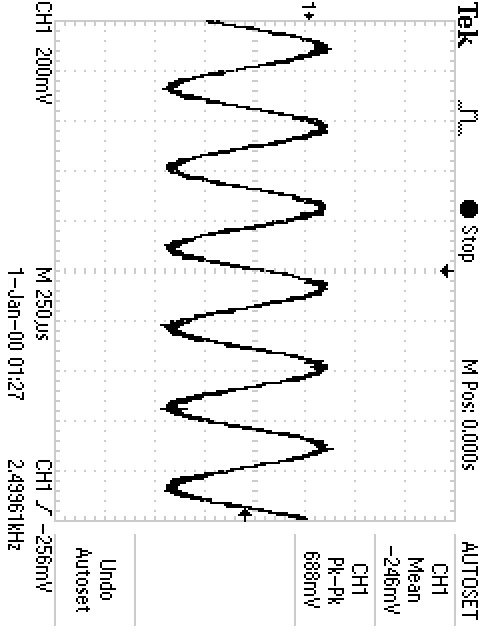
\includegraphics[angle=90,width=1\linewidth]{img/F0009TEK.JPG}} Sin сигнал з $\omega=2.5 kHz$ \\
	\end{minipage}
	\hfill
	\begin{minipage}[h]{0.47\linewidth}
		\center{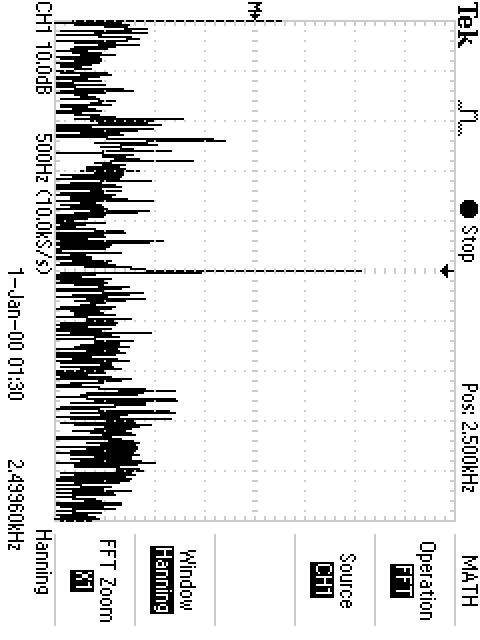
\includegraphics[angle=90,width=1\linewidth]{img/F0010TEK.JPG}} FFT для Sin сигналу з $\omega=2.5 kHz$ \\
	\end{minipage}
	\vfill
	\begin{minipage}[h]{0.47\linewidth}
		\center{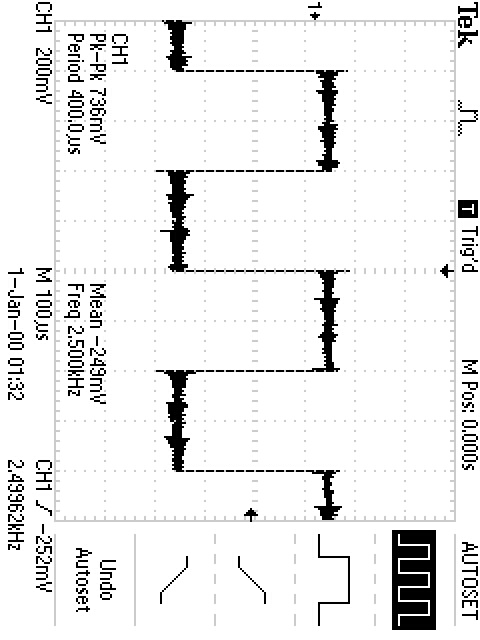
\includegraphics[angle=90,width=1\linewidth]{img/F0011TEK.JPG}} Квадратний сигнал з $\omega=2.5 kHz$\\
	\end{minipage}
	\hfill
	\begin{minipage}[h]{0.47\linewidth}
		\center{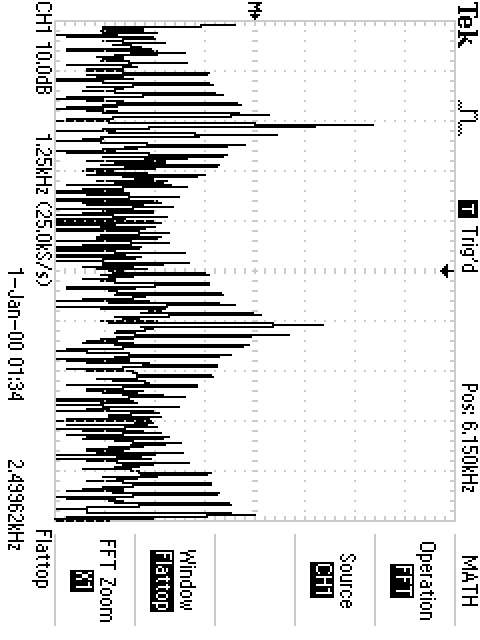
\includegraphics[angle=90,width=1\linewidth]{img/F0012TEK.JPG}} FFT для квадратного сигналу\\
	\end{minipage}
	\vfill
	\begin{minipage}[h]{0.47\linewidth}
		\center{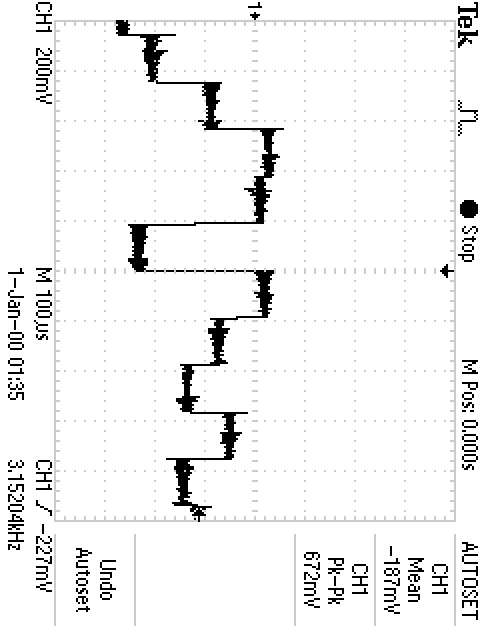
\includegraphics[angle=90,width=1\linewidth]{img/F0013TEK.JPG}} ШІМ шум\\
	\end{minipage}
	\hfill
	\begin{minipage}[h]{0.47\linewidth}
		\center{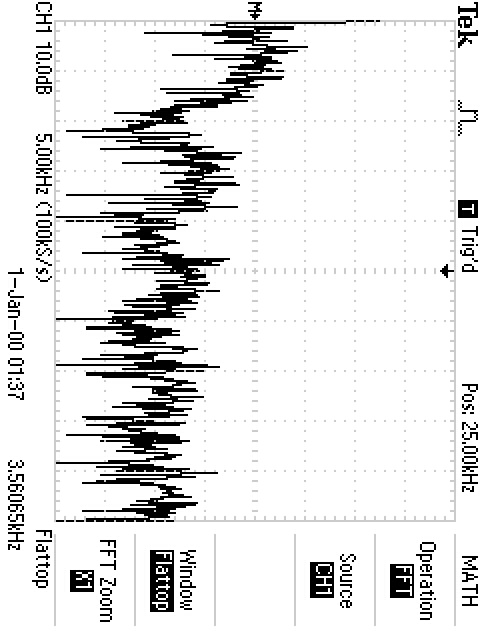
\includegraphics[angle=90,width=1\linewidth]{img/F0014TEK.JPG}} FFT для ШІМ шуму\\
	\end{minipage}
	\caption{Картинки, отримані на екрані осцилографа, за допомогою невідомого генератору.}
	\label{fig:part1}
\end{figure}

\section{Двоканальний режим роботи осцилографа. Побудова фігур Ліссажу.}

Для цієї частини лабораторної роботи нам був необхідний ще один генератор. Тому було прийняте рішення нагло взяти те, що погано лежить, а саме, генератор DDS 9850 під керуванням Arduino Nano (див \cite{lab3}). Дуже швидко ми зрозуміли, що \sout{біда приходить звідки не чекають} осцилограф не вміє записувати на USB накопичувач картинки у режимі ХУ. Тому було прийняти рішення, записати на накопичувач сигнали у виді х(t) та y(t), а потім, використовуючи фраємворк cern ROOT \cite{root}, скомпонувати їх. Відповідні результати зоображені на рис. \ref{fig:part2},\ref{fig:part22}.

\begin{figure}[h]
	\begin{minipage}[h]{0.47\linewidth}
		\center{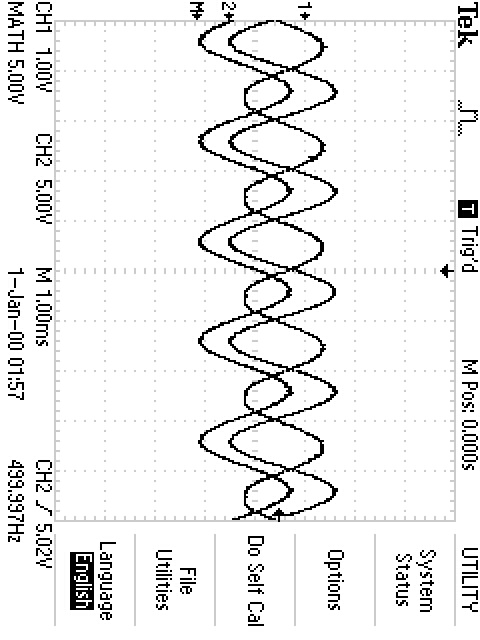
\includegraphics[angle=90,width=1\linewidth]{img/lis/F0001TEK.JPG}} Дві синусоїди із близькими частотами $\omega_{12} \approx 500 Hz$\\
	\end{minipage}
	\hfill
	\begin{minipage}[h]{0.47\linewidth}
		\center{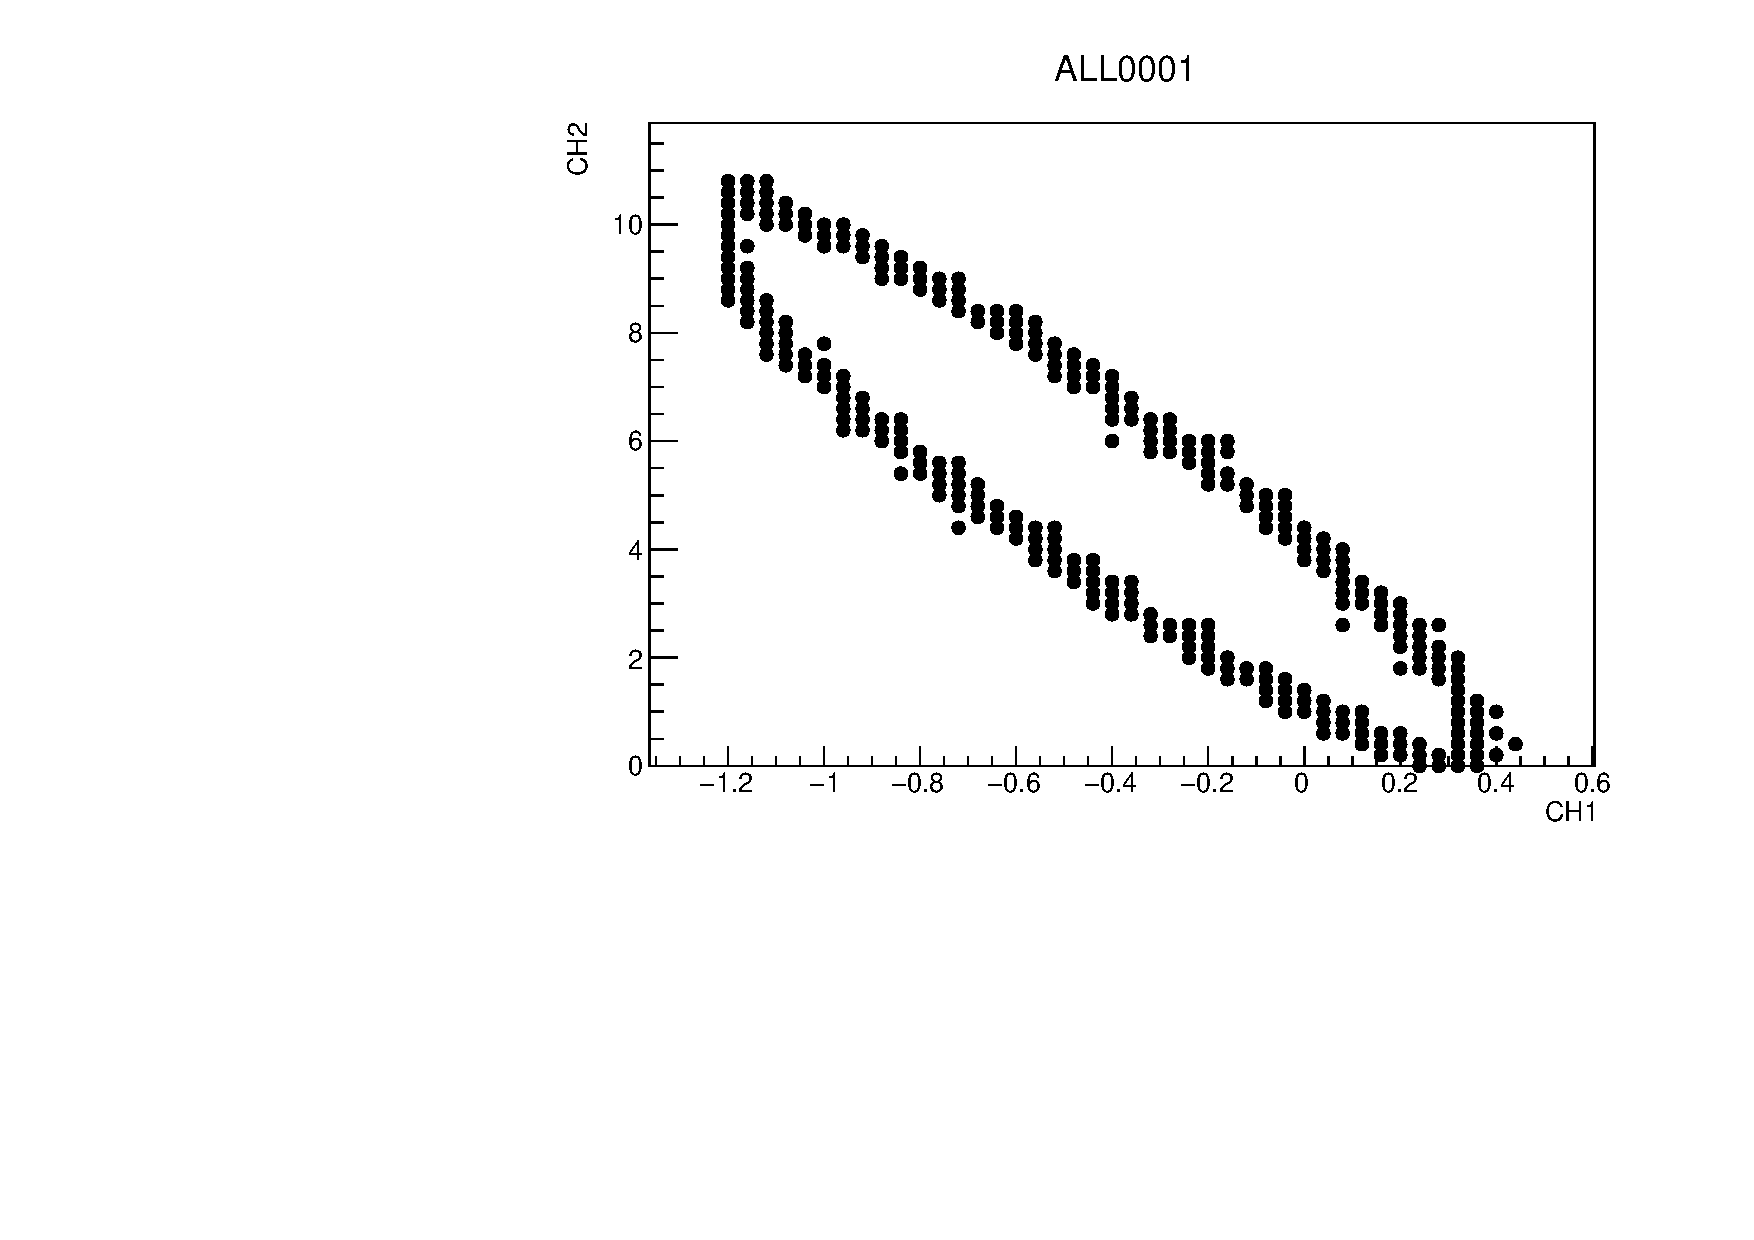
\includegraphics[width=1\linewidth]{img/lis/ALL0001_.pdf}} Відповідна фігура Ліссажу.\\
	\end{minipage}
	\vfill
	\begin{minipage}[h]{0.47\linewidth}
		\center{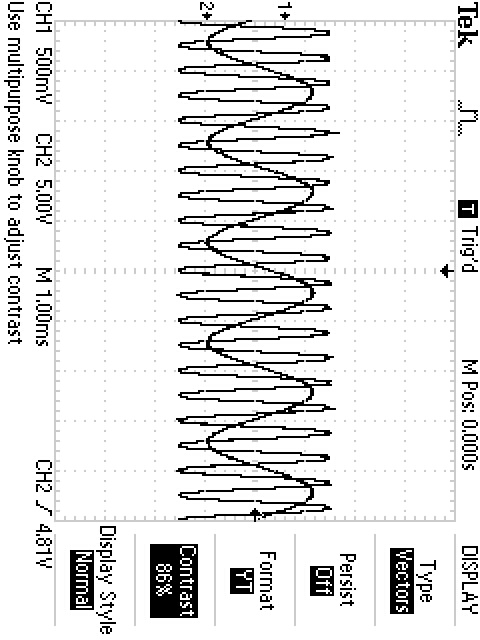
\includegraphics[angle=90,width=1\linewidth]{img/lis/F0002TEK.JPG}} Sin, $\omega_1 = 500Hz$, $\omega_2 = 2.5kHz$\\
	\end{minipage}
	\hfill
	\begin{minipage}[h]{0.47\linewidth}
		\center{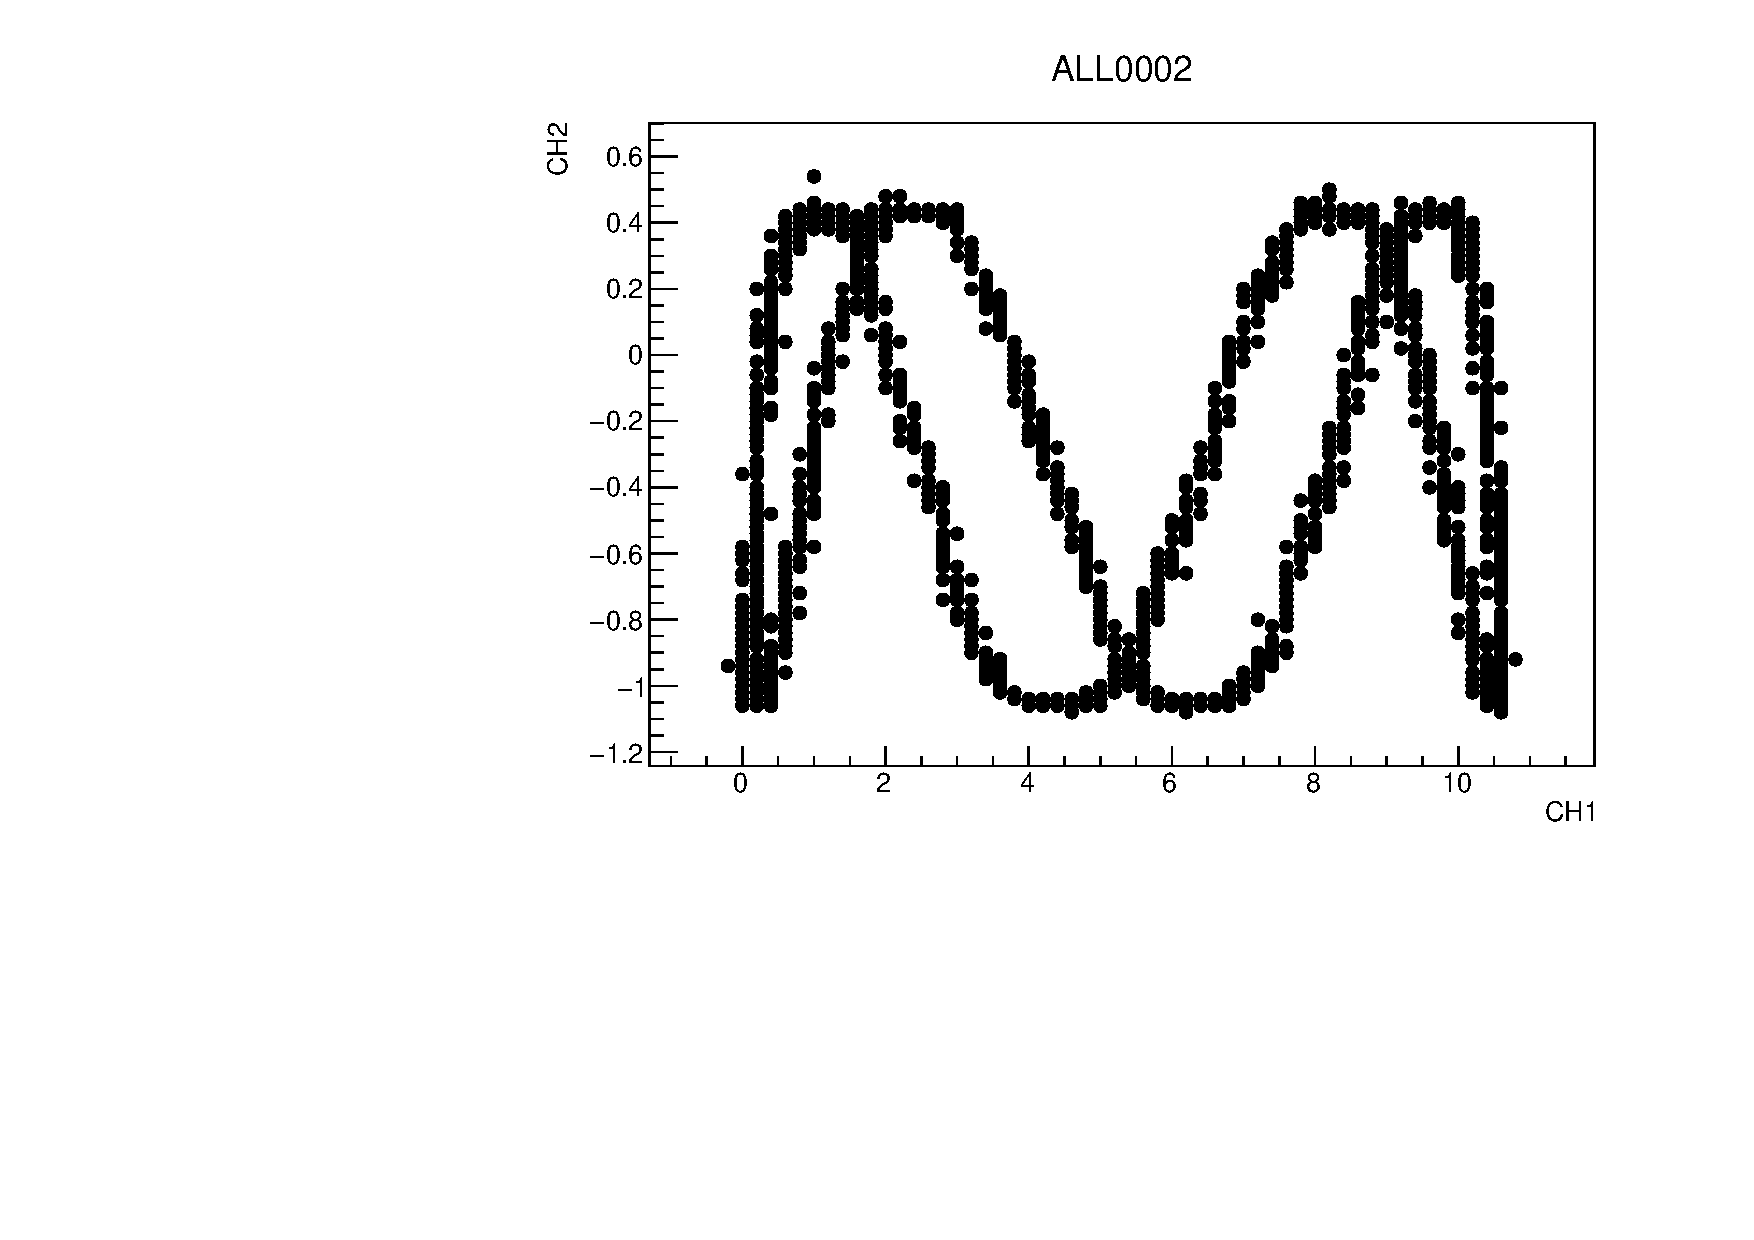
\includegraphics[width=1\linewidth]{img/lis/ALL0002_.pdf}} Відповідна фігура Ліссажу\\
	\end{minipage}
	\vfill
	\begin{minipage}[h]{0.47\linewidth}
		\center{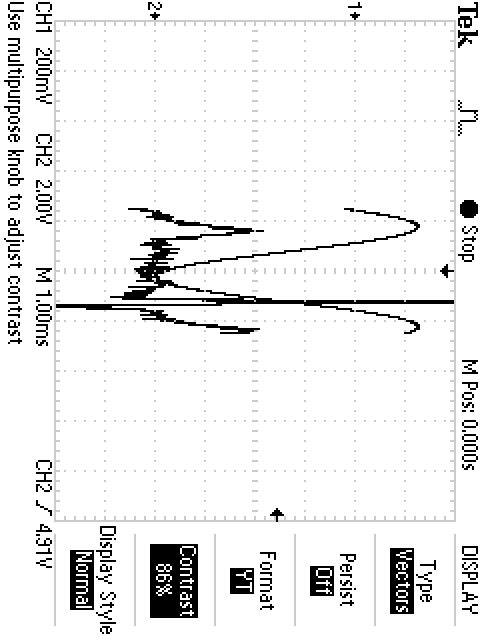
\includegraphics[angle=90,width=1\linewidth]{img/lis/F0006TEK.JPG}} Кардіограма + Sin ($\omega = 500Hz$) \\
	\end{minipage}
	\hfill
	\begin{minipage}[h]{0.47\linewidth}
		\center{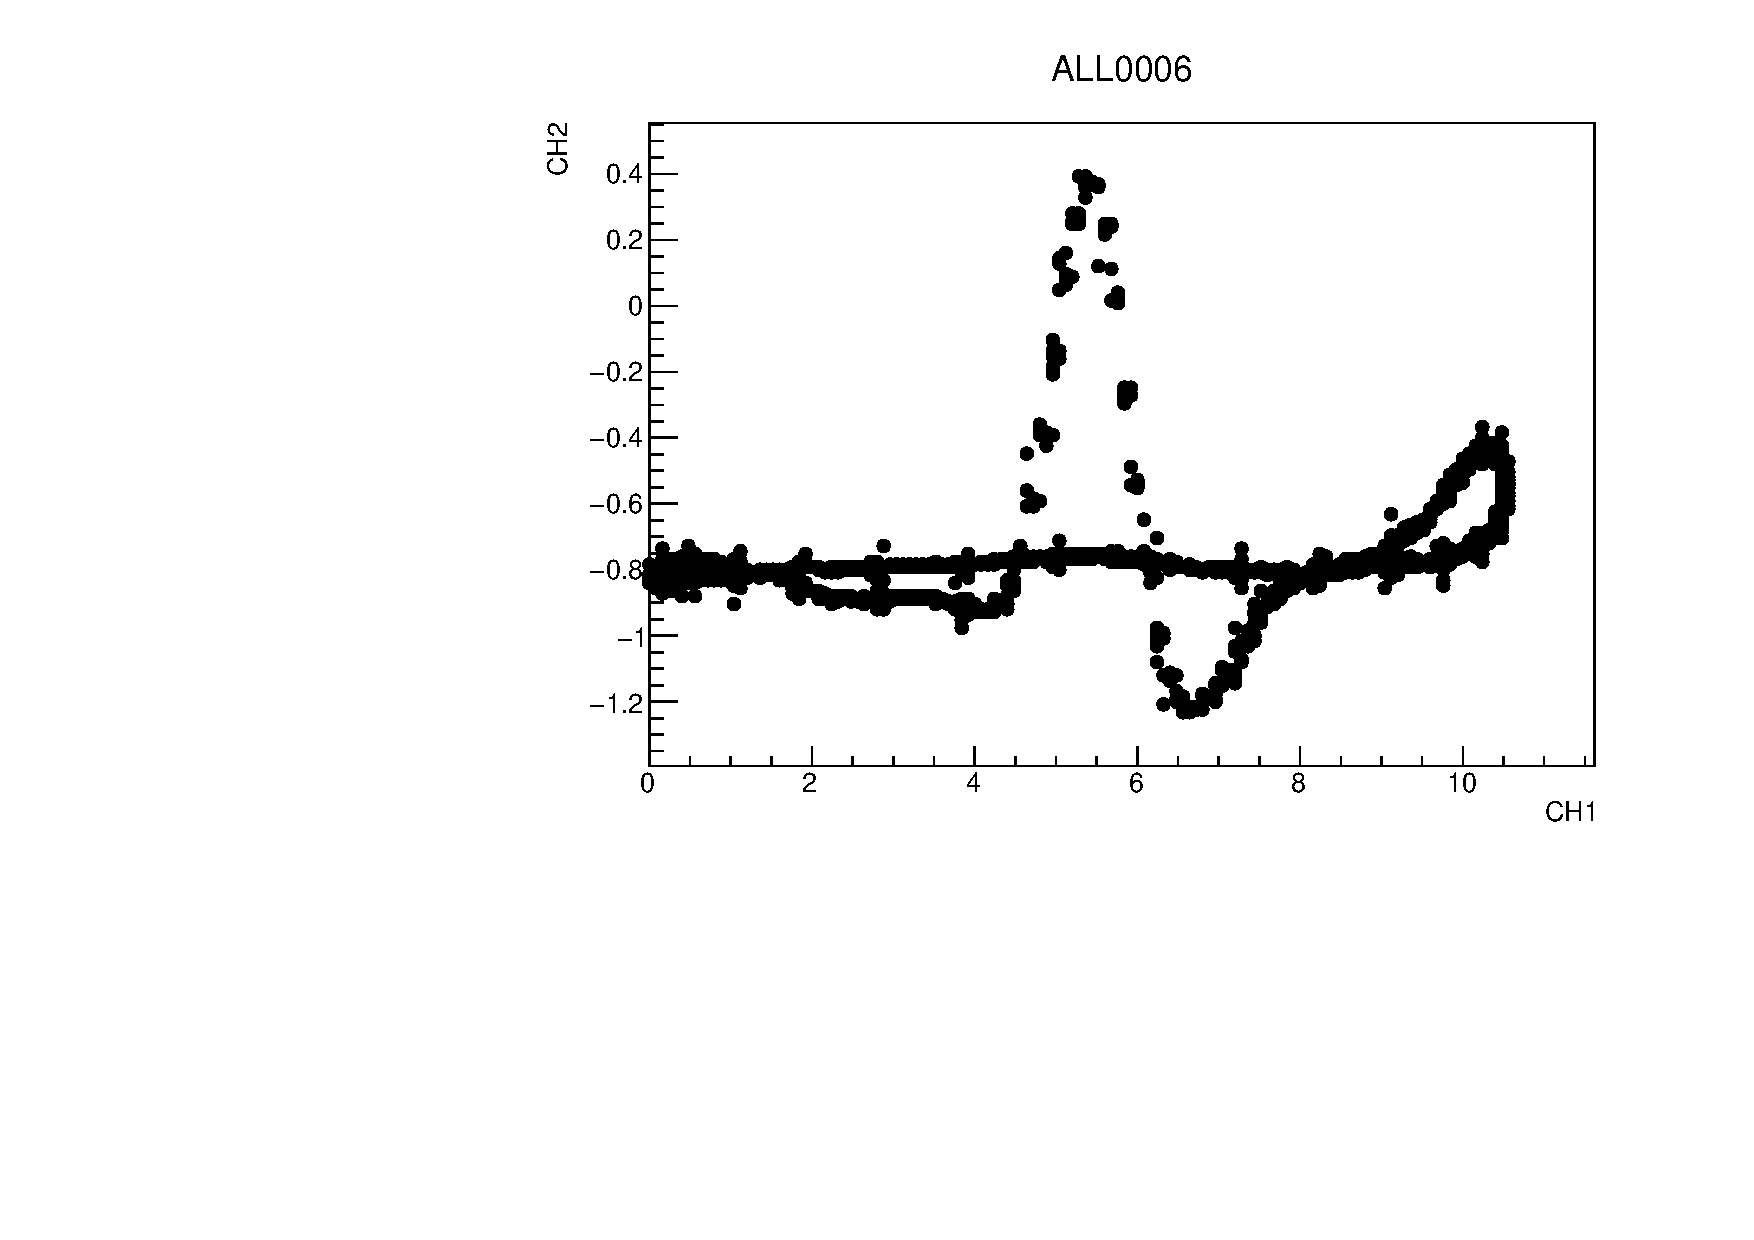
\includegraphics[width=1\linewidth]{img/lis/ALL0006_.pdf}} Відповідна фігура Ліссажу \\
	\end{minipage}
	\caption{Картинки, отримані на екрані осцилографа, за допомогою невідомого генератору та DDS9850}
	\label{fig:part2}
\end{figure}

\begin{figure}[h]
	\begin{minipage}[h]{0.47\linewidth}
		\center{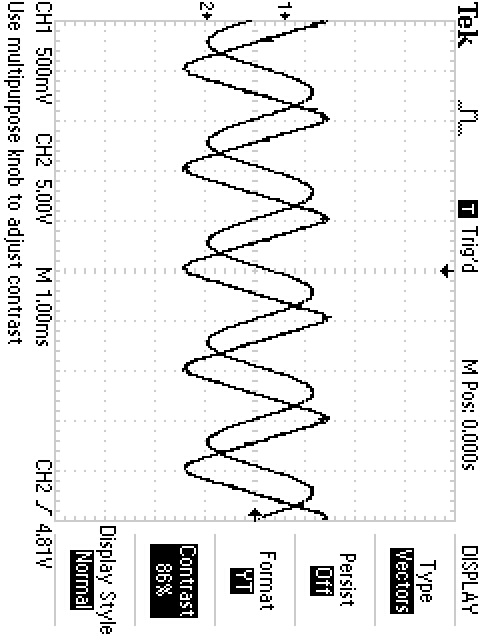
\includegraphics[angle=90,width=1\linewidth]{img/lis/F0003TEK.JPG}} Sin ($\omega=500 Hz$) + трикутний ($\omega=500 Hz$) \\
	\end{minipage}
	\hfill
	\begin{minipage}[h]{0.47\linewidth}
		\center{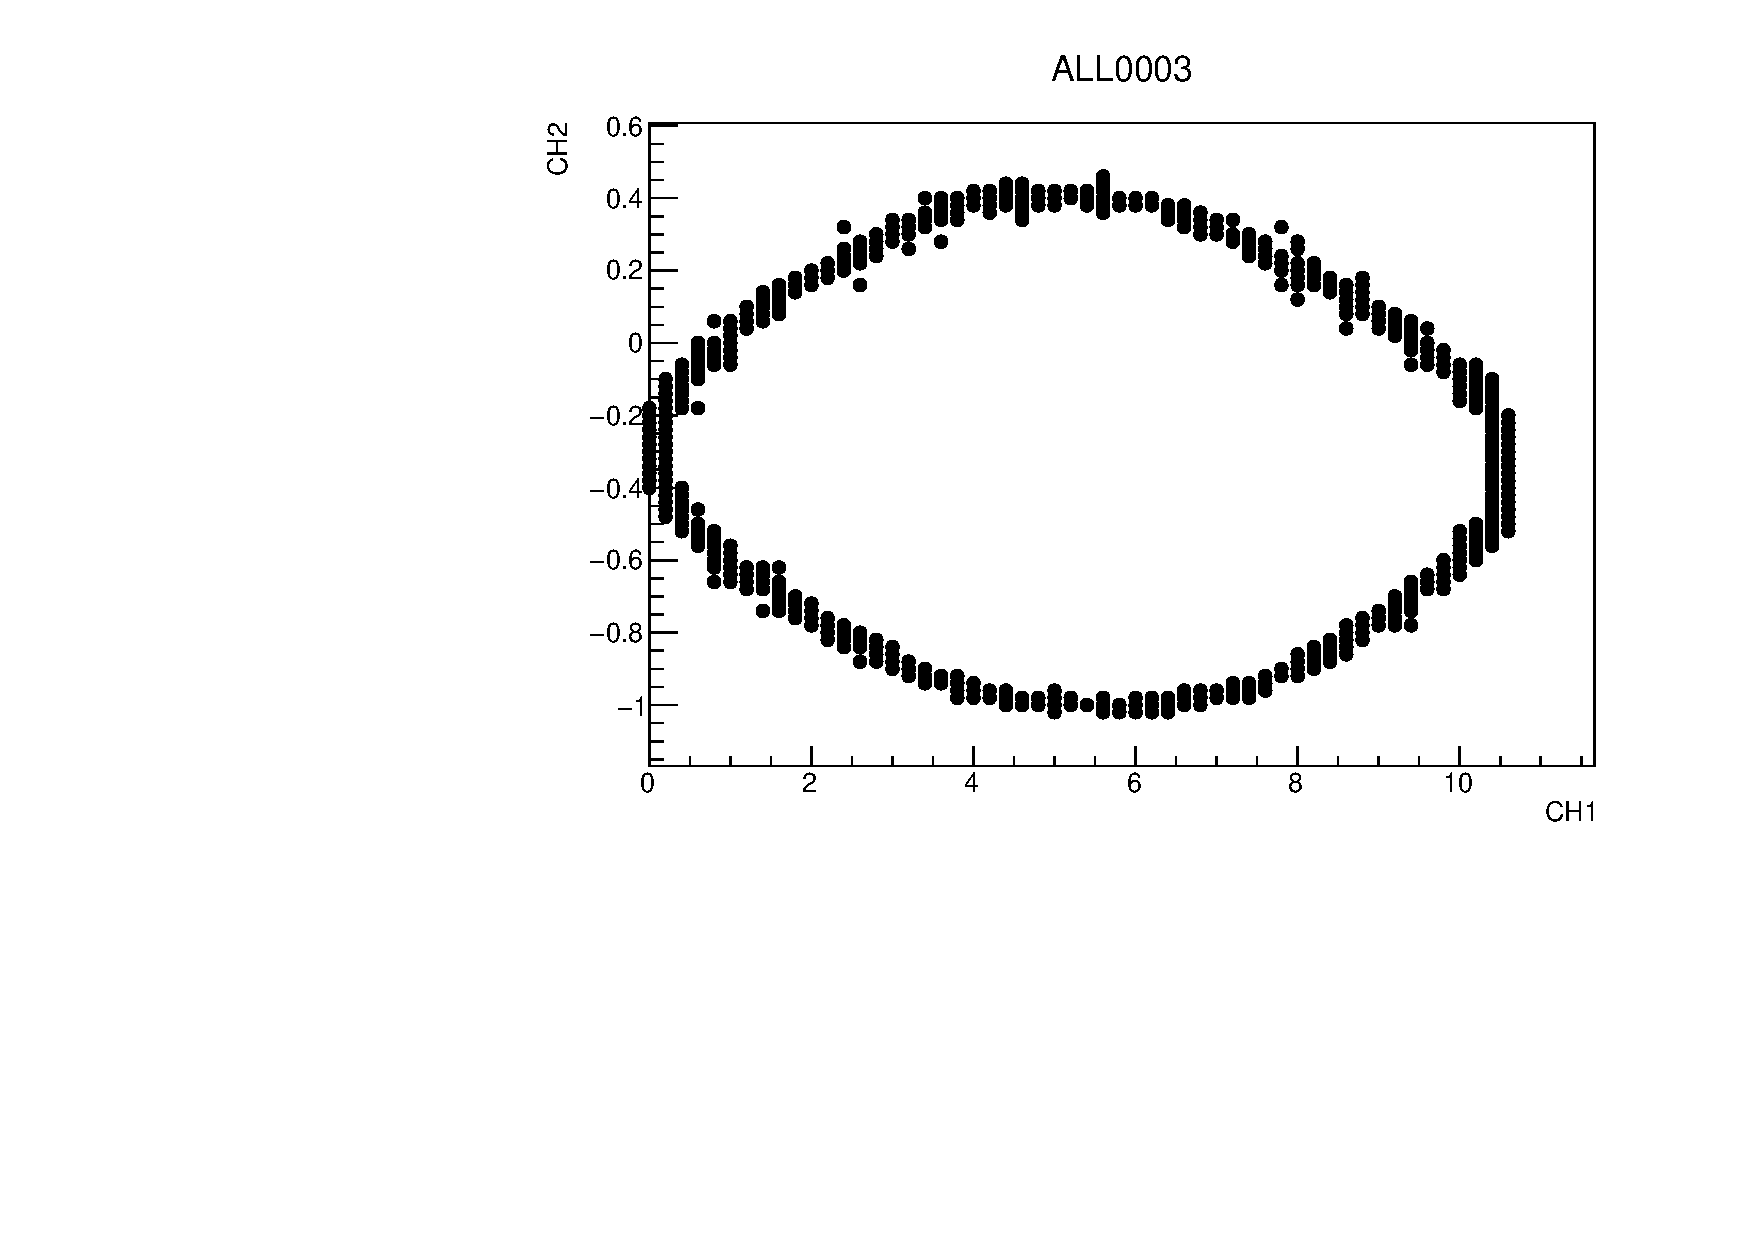
\includegraphics[width=1\linewidth]{img/lis/ALL0003_.pdf}} Відповідна фігура Ліссажу \\
	\end{minipage}
	\vfill
	\begin{minipage}[h]{0.47\linewidth}
		\center{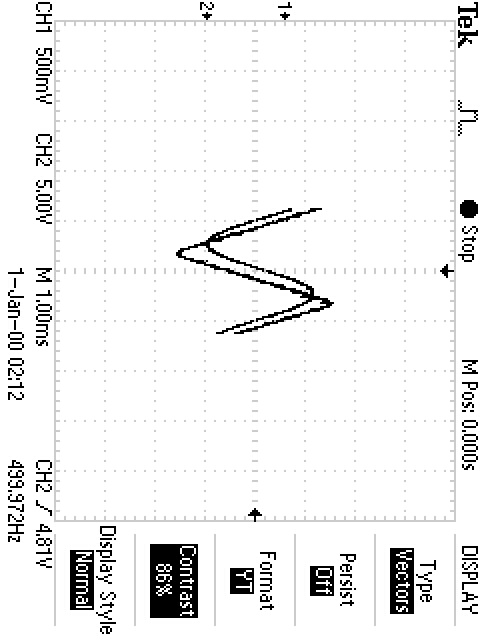
\includegraphics[angle=90,width=1\linewidth]{img/lis/F0004TEK.JPG}} Sin ($\omega=500 Hz$) + трикутний ($\omega=500 Hz$) \\
	\end{minipage}
	\hfill
	\begin{minipage}[h]{0.47\linewidth}
		\center{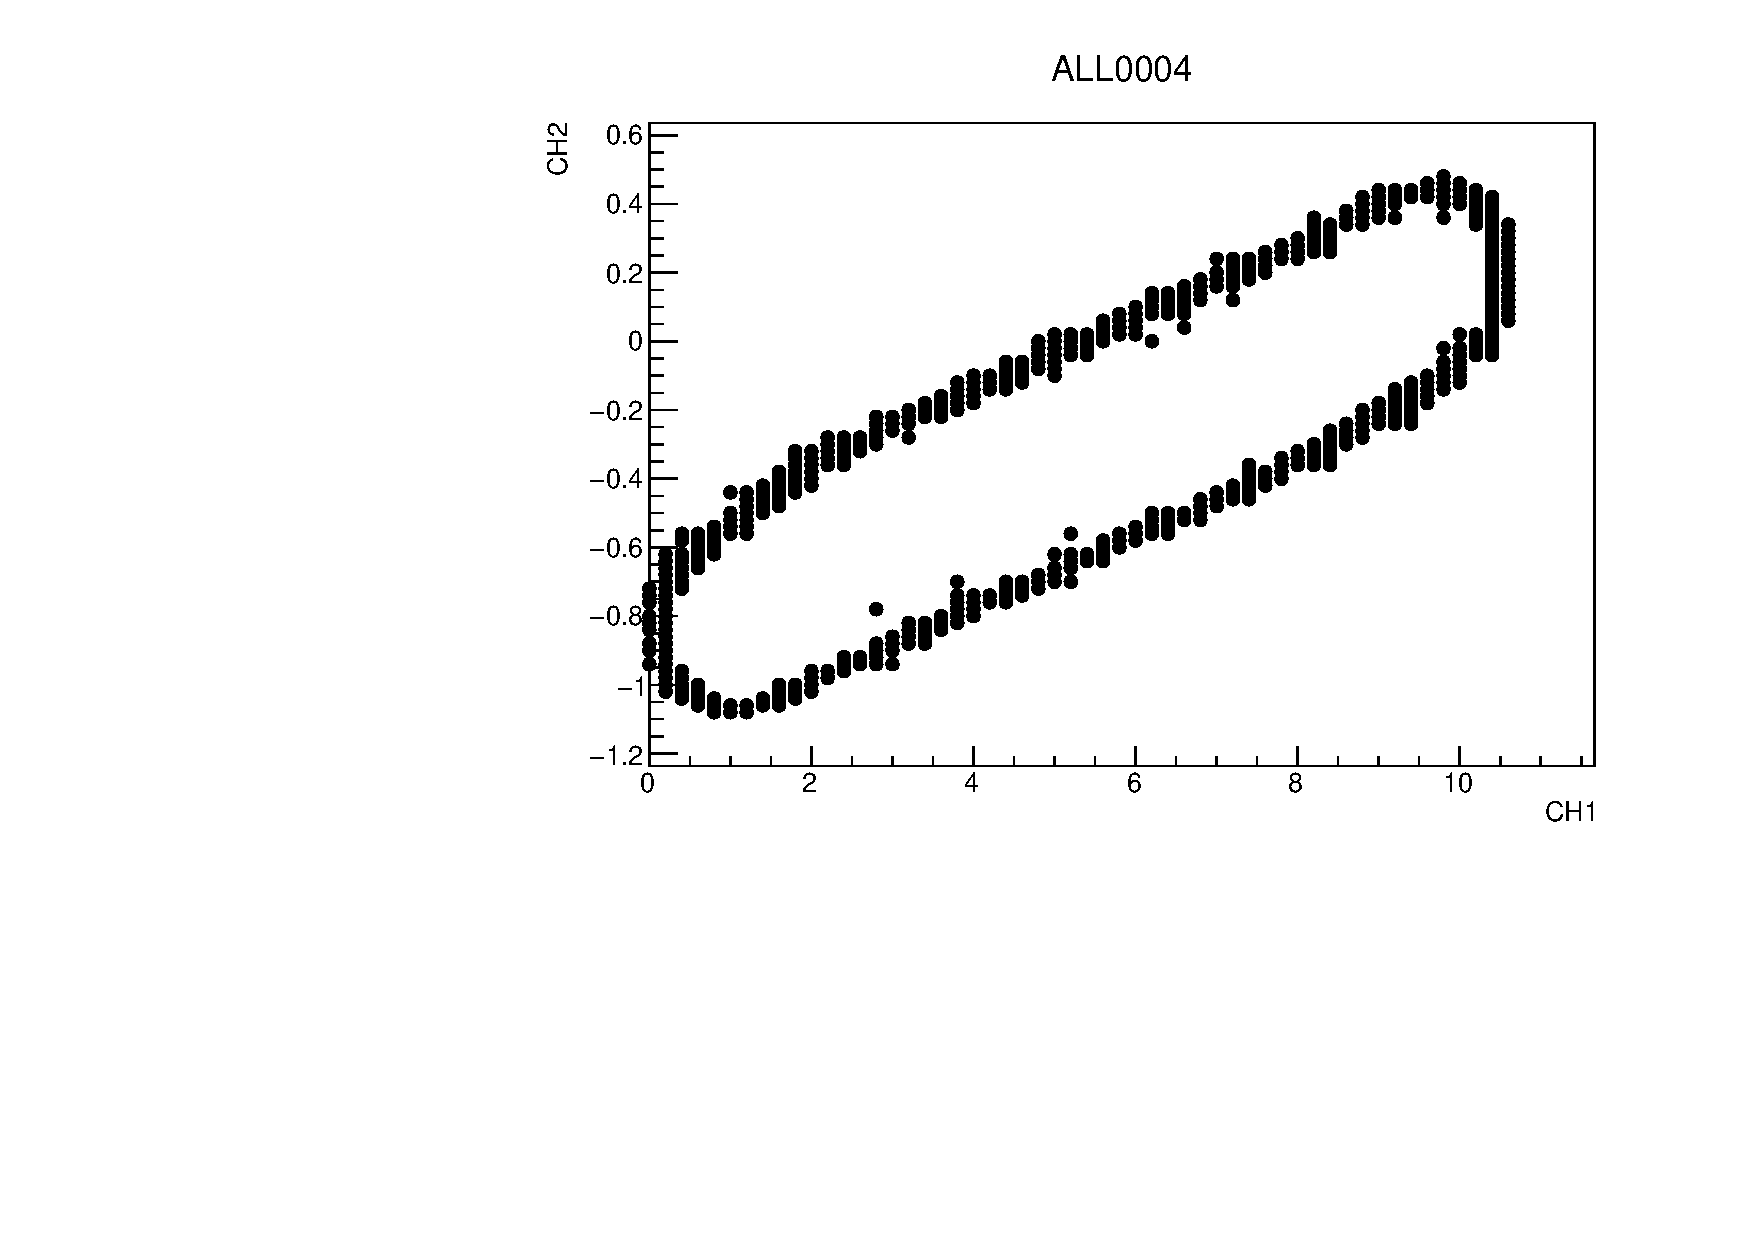
\includegraphics[width=1\linewidth]{img/lis/ALL0004_.pdf}} Відповідна фігура Ліссажу \\
	\end{minipage}
	\vfill
	\begin{minipage}[h]{0.47\linewidth}
		\center{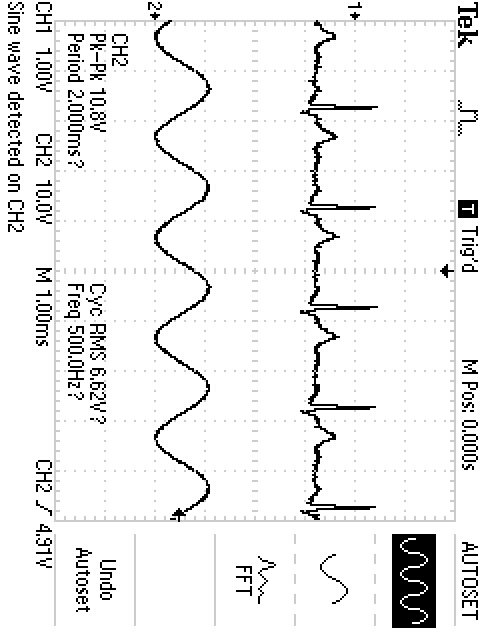
\includegraphics[angle=90,width=1\linewidth]{img/lis/F0005TEK.JPG}} Кардіограма + синусоїда ($\omega = 500Hz$)\\
	\end{minipage}
	\hfill
	\begin{minipage}[h]{0.47\linewidth}
		\center{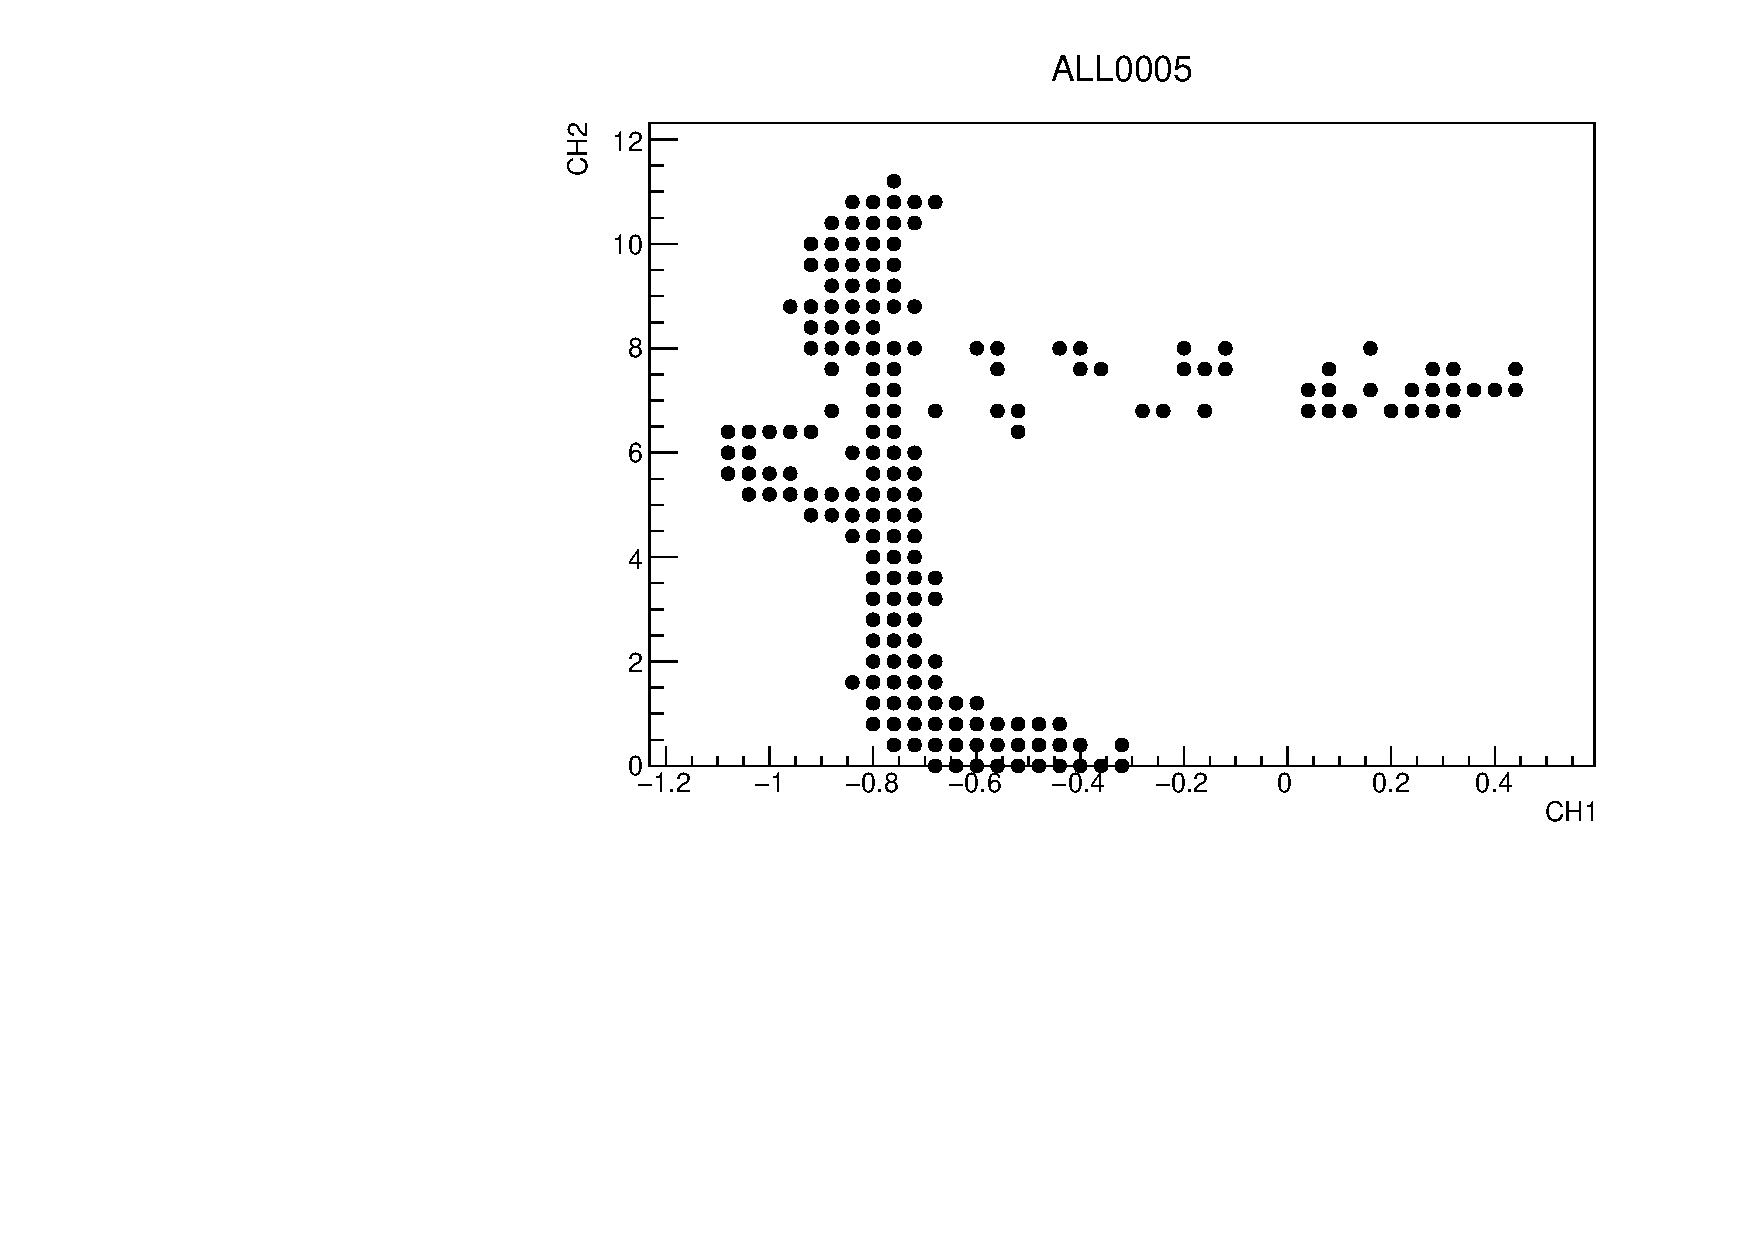
\includegraphics[width=1\linewidth]{img/lis/ALL0005_.pdf}} Відповідна фігура Ліссажу \\
	\end{minipage}
	\caption{Картинки, отримані на екрані осцилографа, за допомогою невідомого генератору та DDS9850}
	\label{fig:part22}
\end{figure}

